\documentclass{beamer}
\mode<presentation> {
\usetheme{Madrid}
}

\usepackage{amsmath,amsthm,amssymb,amsfonts,listings,graphicx,caption,subcaption,hyperref,mathtools} % Allows including images
\usepackage{booktabs} % Allows the use of \toprule, \midrule and \bottomrule in tables

%-----------------------------------------------------------
%	TITLE PAGE
%-----------------------------------------------------------

\title[Missing Data]{Monday Group Presentation on Missing Data} % The short title appears at the bottom of every slide, the full title is only on the title page

\author{Sam Shi} % Your name
\institute[Ryerson] % Your institution as it will appear on the bottom of every slide, may be shorthand to save space
{
Ryerson University \\ % Your institution for the title page
\medskip
%\textit{john@smith.com} % Your email address
}
\date{\today} % Date, can be changed to a custom date

\begin{document}

\begin{frame}
\titlepage % Print the title page as the first slide
\end{frame}

\begin{frame}
\frametitle{Overview} % Table of contents slide, comment this block out to remove it
\tableofcontents % Throughout your presentation, if you choose to use \section{} and \subsection{} commands, these will automatically be printed on this slide as an overview of your presentation
\end{frame}

%----------------------------------------------------------------------------------------
%	PRESENTATION SLIDES
%----------------------------------------------------------------------------------------

%------------------------------------------------
\section{Missing data} % Sections can be created in order to organize your presentation into discrete blocks, all sections and subsections are automatically printed in the table of contents as an overview of the talk
%------------------------------------------------

\subsection{Types of Missing Data} % A subsection can be created just before a set of slides with a common theme to further break down your presentation into chunks

\begin{frame}
\frametitle{Types of Missing Data}

supposed you want to model weight $Y$ as a function of gender $X$ and you do a survey asking for $Y$ and $X$, in the end there are some missing values(data point missing or data attribute missing), below are possible scenarios,
\begin{itemize}
\item{Missing completely at random(MCAR)}\\
No particular reasons why the data is missing, such as, it can be someone dropped the survey paper, hardly recognizable hand-writing, etc. (data are rarely MCAR) 
\item{Missing at random(MAR)}\\
It can happen that one gender $X$ would less likely to disclose their weight information than the other.
\item{Missing not at random(MNAR)}\\
Missing value itself is related to why it is missing, e.g. a person with higher weight $Y$ would more likely not fill out the weight blank on survey. 
\end{itemize}
\end{frame}

%------------------------------------------------
\subsection{Why it is important}
\fontsize{6pt}{7.2}\selectfont
\begin{frame}
\frametitle{why it is important}
\begin{itemize}
\item {Easy to occur very common}
\begin{figure}[h!]
	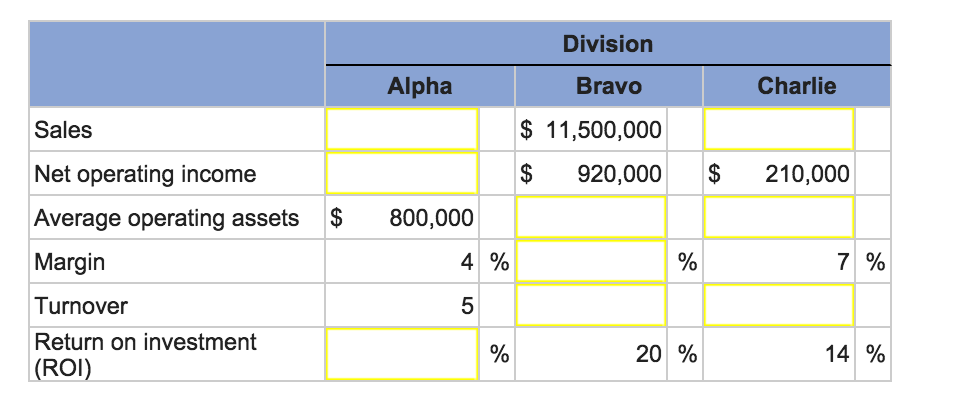
\includegraphics[width=0.2\textwidth]{missing.png}
\end{figure}
\item  Nearly all standard statistical methods presume complete information for
all the variables included in the analysis; Machine learning models need to have complete input.\cite{p1}
\begin{figure}[h!]
	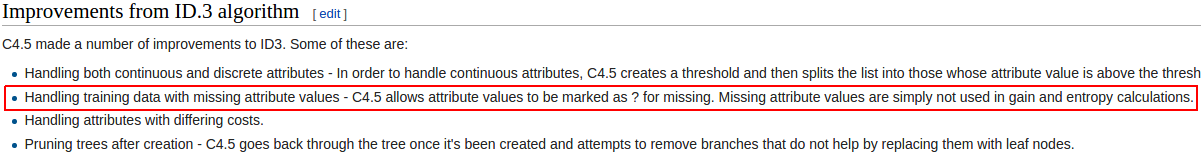
\includegraphics[width=0.6\textwidth]{c45.png}
\end{figure}
\item Create bias \cite{p2}
\begin{figure}[h!]
	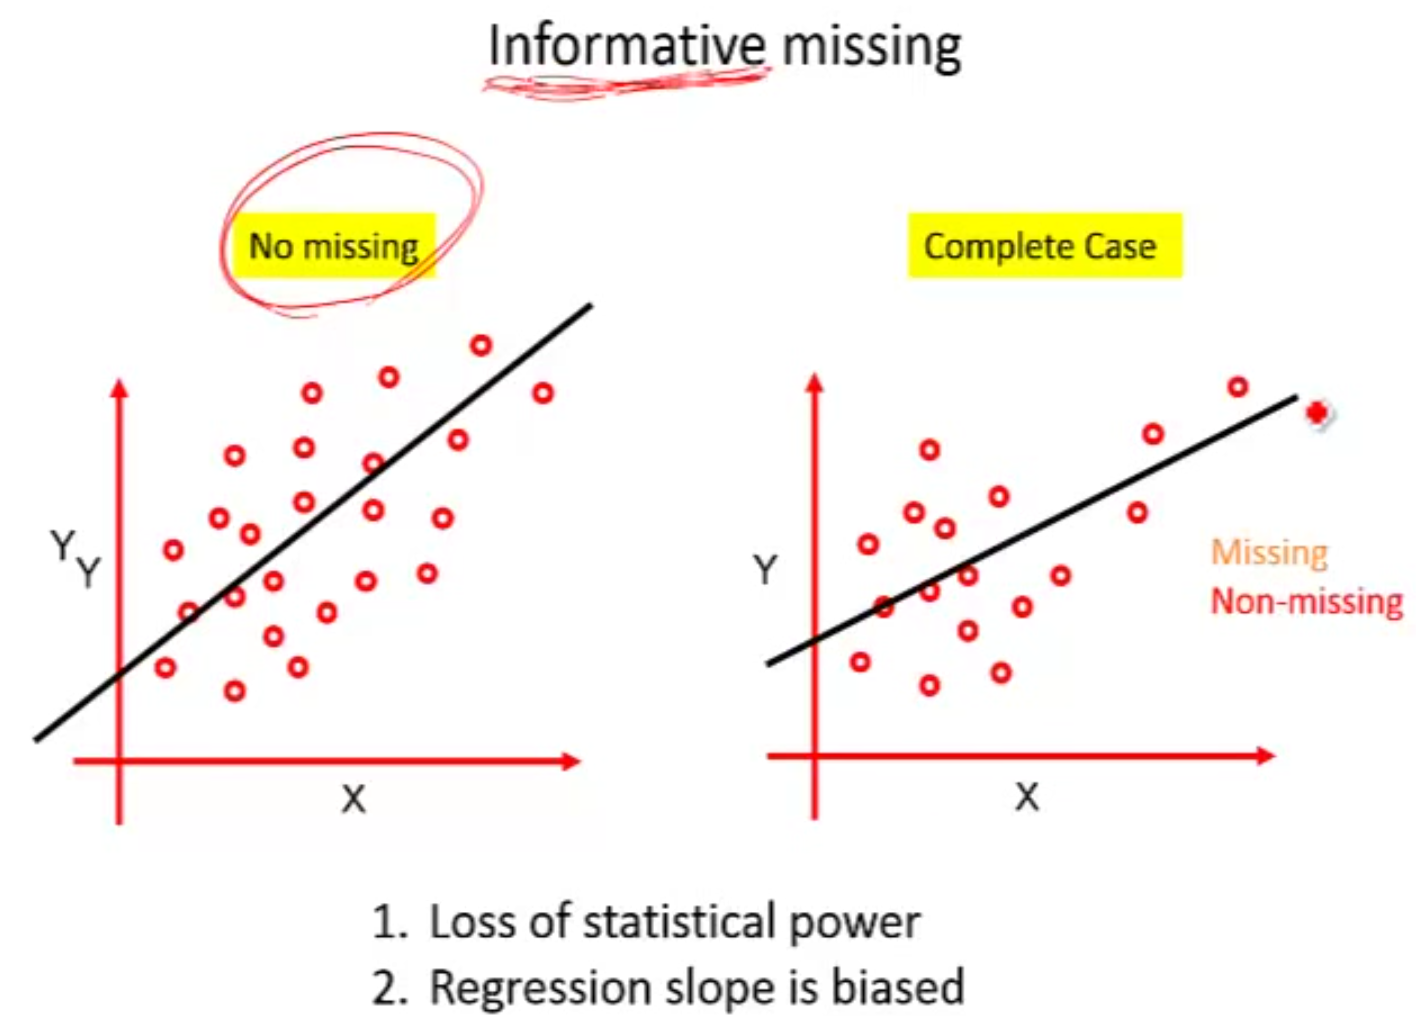
\includegraphics[width=0.5\textwidth]{bias.png}
\end{figure}
\end{itemize}
\end{frame}

%------------------------------------------------
\subsection{Common ways to deal with missing data}
\fontsize{11pt}{7.2}\selectfont
\begin{frame}
\frametitle{Common ways to deal with missing data}
A quick summary before we introduce some methods, \cite{p3}\\
	\begin{itemize}
		\item Listwise deletion (or complete case analysis)
		\item Imputation methods
		\item Multiple Imputation
		\item Maximum Likelihood 
		\item Bayesian simulation methods
		\item Hot deck imputation methods
	\end{itemize}
\end{frame}
%------------------------------------------------

\section{Methods}
\subsection{Listwise deletion}
%------------------------------------------------
\begin{frame}{Listwise deletion}
\begin{columns}[c] 
	
\column{.5\textwidth} % Left column and width
\begin{figure}[h!]
	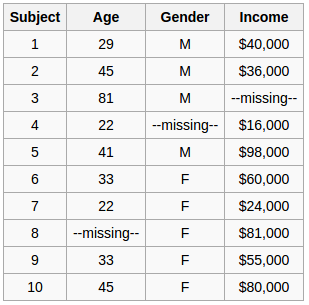
\includegraphics[width=\textwidth]{listwise.png}
\end{figure}
-- picture from Wiki
\column{.5\textwidth} % Right column and width
\textbf{Advantage}:\\
\begin{itemize}
\item{Easy to implement, no special computation method requires}
\item{It is valid if the missing data is MCAR}
\item{If the proportion of deleted data is small, e.g. $<5\%$}
\end{itemize}
\textbf{Disadvantage}:\\
\begin{itemize}
	\item{Can exclude a large portion of data}
	\item{Missing data are MCAR rarely happens in reality}
	\item{Introduce bias}
\end{itemize}
\end{columns}


\end{frame}
%------------------------------------------------
\subsection{Single imputation}
\begin{frame}{Imputation}
\textbf{(Unconditional) Mean imputation}: Use mean value of available data to represent missing data.
\begin{itemize}
\item Easy to implement, mean stays the same; 
\item Decreased variance and introduce bias. 
\end{itemize}
\textbf{Conditional mean imputation}: Suppose we want to build an regression model with multiple attributes, and there are some missing values in one of the attribute $a_i$, then we use all data with avaliable attributes to perform regression on $a_i$. 
\begin{itemize}
\item{Conditional mean imputations may generate accurate predictions, the uncertainty or imputation error is estimated at all.}
\end{itemize}
(KNN)
\end{frame}
%------------------------------------------------
\subsection{Multiple imputation}
\begin{frame}{Multiple imputation} 
Multiple Imputation through Chained Equations(MICE):\\
\-\ \\
\underline{Fill in the missing data with random draws from the observed values.}\\
\-\ \\
	\begin{tabular}{| c | c | c | c | c |} %l for left align
		\hline
		a & b & c & d & y \\ %[1.5ex] 
		\hline
		2 & 3 & 8 & -1 & 0 \\ 
		\boxed{?} & 2.5 & 12 & -1 & 1 \\
		4 & 4 & -1.5 & 0 & 0 \\
		-5 & 3 & \boxed{?} & 1.2 & 1 \\
		0.5 & 3 & 8 & -0.5 & 0 \\
		7 & 9.2 & \boxed{?} & 1 & 1 \\
		\hline
	\end{tabular}
$\xRightarrow[\text{mean impute}]{\text{Initialize randomly}}$
\begin{tabular}{| c | c | c | c | c |} %l for left align
	\hline
	a & b & c & d & y \\ %[1.5ex] 
	\hline
	2 & 3 & 8 & -1 & 0 \\ 
	\boxed{2} & 2.5 & 12 & -1 & 1 \\
	4 & 4 & -1.5 & 0 & 0 \\
	-5 & 3 & \boxed{0} & 1.2 & 1 \\
	0.5 & 3 & 8 & -0.5 & 0 \\
	7 & 9.2 & \boxed{4} & 1 & 1 \\
	\hline
\end{tabular}
\vspace*{\fill}
\end{frame}
%------------------------------------------------
\begin{frame}{Multiple imputation}
\underline{Move through the columns of variables and perform single‐variable}
\underline{ imputation using some method}\\
\-\ \\
\begin{columns}[c]
\column{0.5\textwidth}
\begin{tabular}{| c | c | c | c | c |} %l for left align
	\hline
	a & b & c & d & y \\ %[1.5ex] 
	\hline
	2 & 3 & 8 & -1 & 0 \\ 
	\boxed{2} & 2.5 & 12 & -1 & 1 \\
	4 & 4 & -1.5 & 0 & 0 \\
	-5 & 3 & \boxed{0} & 1.2 & 1 \\
	0.5 & 3 & 8 & -0.5 & 0 \\
	7 & 9.2 & \boxed{4} & 1 & 1 \\
	\hline
\end{tabular}
\column{0.5\textwidth}
we perform regression on each column, starting with attribute $a$ using the values of all the rest attribute with filled in values:
\begin{equation*}
a \sim b + c + d + y
\end{equation*}
suppose this gives us a new value $\hat{a}=-3$, then we update it and keep doing the same for the other attribute, $c$
\end{columns}
\end{frame}
%------------------------------------------------
\begin{frame}{Multiple imputation}
\underline{repeat until a number of iteration converged}\\

\begin{columns}[c]
\column{0.5\textwidth}
\begin{tabular}{| c | c | c | c | c |} %l for left align
		\hline
		a & b & c & d & y \\ %[1.5ex] 
		\hline
		2 & 3 & 8 & -1 & 0 \\ 
		\boxed{-3} & 2.5 & 12 & -1 & 1 \\
		4 & 4 & -1.5 & 0 & 0 \\
		-5 & 3 & \boxed{0} & 1.2 & 1 \\
		0.5 & 3 & 8 & -0.5 & 0 \\
		7 & 9.2 & \boxed{4} & 1 & 1 \\
		\hline
\end{tabular}
\column{0.5\textwidth}
now we want perform regression on $c$ using the newly updated $\hat{a}$:
\begin{equation*}
	c \sim \hat{a} + b + d + y
\end{equation*}
then we will obtain a new $\hat{c}$. \\
\-\ \\
Iterate certain number of times or set up a convergence limit. \\
\-\ \\Finally we do all above steps $m$ times each with different filled in values, and obtain $m$ imputed data sets.
\end{columns}
\end{frame}
%------------------------------------------------
\begin{frame}{Multiple imputation(PMM)}
Previous slides we talked about simple linear regression method, but there are many ways to do multiple imputation, and the default one R MICE uses is \textit{Predictive Mean Matching} (PMM).
\begin{columns}[c]
	\column{0.5\textwidth}
	\begin{tabular}{| c | c | c | c | c |} %l for left align
		\hline
		a & b & c & d & y \\ %[1.5ex] 
		\hline
		2 & 3 & 8 & -1 & 0 \\ 
		\boxed{?} & 2.5 & 12 & -1 & 1 \\
		4 & 4 & -1.5 & 0 & 0 \\
		-5 & 3 & \boxed{0} & 1.2 & 1 \\
		0.5 & 3 & 8 & -0.5 & 0 \\
		7 & 9.2 & \boxed{4} & 1 & 1 \\
		\hline
	\end{tabular}
	\column{0.5\textwidth}
	we still start with regression on $a$ using avaliable data with filled in data:
	\begin{equation*}
	a \sim b + c+ d + y
	\end{equation*}
	then we obtain a new $\hat{a}$ vector $[3.5, 2, 5, -3, 0, 6]$. \\
	\-\ \\
	we pick 3 the closest values (in terms of distance e.g. Euclidiean) and randomly choose one of them as the fill-in value. 
\end{columns}


\end{frame}


%------------------------------------------------
\begin{frame}{Multiple imputation(PMM)}
	\begin{columns}[c]
		\column{0.5\textwidth}
		\begin{tabular}{| c | c | c | c | c | c |} %l for left align
			\hline
			a & b & c & d & y & $\hat{a}$\\ %[1.5ex] 
			\hline
			2 & 3 & 8 & -1 & 0 & $\underline{3.5}$\\ 
			\boxed{?} & 2.5 & 12 & -1 & 1 & \boxed{2} \\
			4 & 4 & -1.5 & 0 & 0 & $\underline{5}$\\
			-5 & 3 & \boxed{0} & 1.2 & 1 & -3\\
			0.5 & 3 & 8 & -0.5 & 0 & $\underline{0}$\\
			7 & 9.2 & \boxed{4} & 1 & 1 & 6\\
			\hline
		\end{tabular}
		\column{0.5\textwidth}
		so we see $[3.5, 5, 0]$ are three values(you can choose different number of points) that closest to $\hat{a}=2$, so we ranomly choose one out of their corresponding avaliable data, i.e. $[2, 4, 0.5]$\\
		\-\ \\
		Again, we iterate until satisfied, and repeat this whole process $m$ times each with different initializtion. \\
		\-\ \\
		This is the default multiple imputation method in MICE for continuous
		variables.
	\end{columns}
	
	
\end{frame}
%------------------------------------------------
\begin{frame}{Multiple imputation(PMM)}
	\begin{columns}[c]
		\column{0.5\textwidth}
		\begin{tabular}{| c | c | c | c | c |} %l for left align
			\hline
			a & b & c & d & y \\ %[1.5ex] 
			\hline
			2 & 3 & 8 & -1 & 0 \\ 
			\boxed{3.5} & 2.5 & 12 & -1 & 1 \\
			4 & 4 & -1.5 & 0 & 0 \\
			-5 & 3 & \boxed{12} & 1.2 & 1 \\
			0.5 & 3 & 8 & -0.5 & 0 \\
			7 & 9.2 & \boxed{-1.5} & 1 & 1\\
			\hline
		\end{tabular}
		\column{0.5\textwidth}
		We have obtained one imputated data, then repeat $m$ times, where after you can perform statistical analysis on those $m$ results and you can pool the machine learning parameters from those $m$ results to give you a final model\\
		\-\ \\ 
		Use real data to fill in missing data but we are using our imputation model to pick which one we fill in.
	\end{columns}
\end{frame}
%------------------------------------------------
\begin{frame}{Multiple imputation(PMM)}
\fontsize{6pt}{7.2}\selectfont
\begin{figure}[h!]
	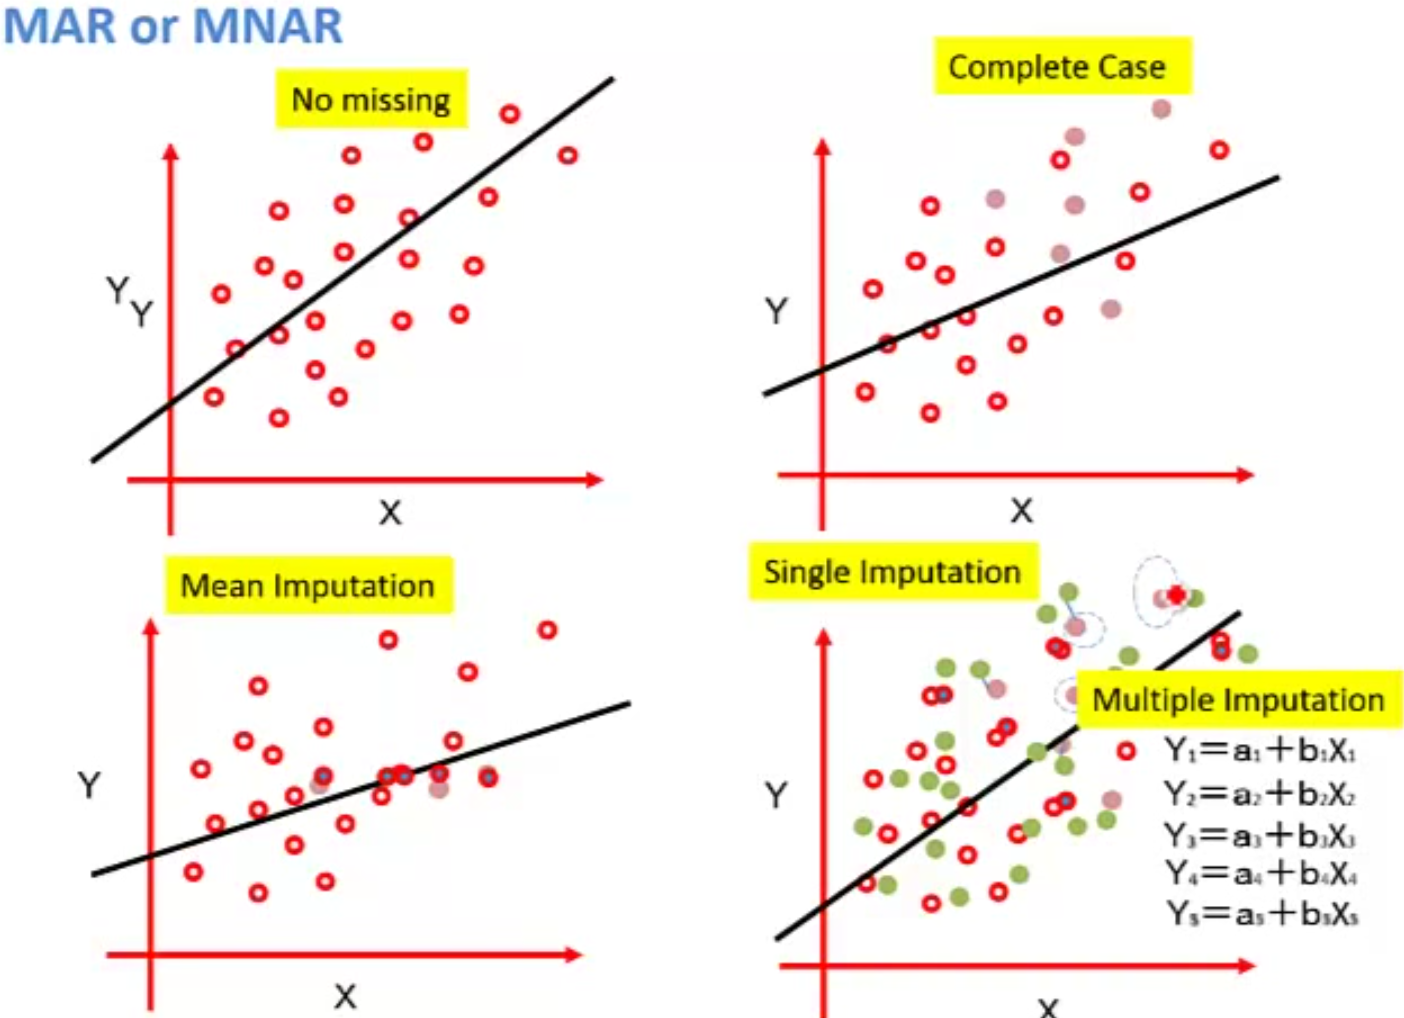
\includegraphics[width=0.4\textwidth]{pmm_result.png}
\end{figure}
More details on Rubin's paper about statistical analysis:\\ \url{http://ww2.amstat.org/sections/SRMS/Proceedings/papers/1988_016.pdf} 
\begin{figure}[h!]
	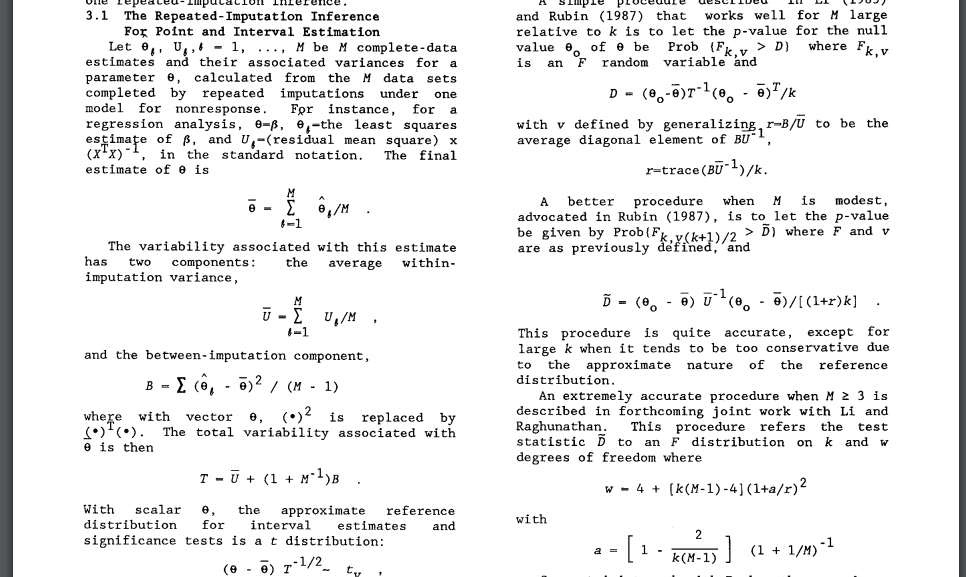
\includegraphics[width=0.4\textwidth]{rubin2.png}
\end{figure}
\end{frame}
%------------------------------------------------
\begin{frame}{Maximum likelihood}
\fontsize{8pt}{7.2}\selectfont
\begin{equation*}
	p(X|\theta) = \prod_{i=1}^{N}p(x_i|\theta) = \prod_{i=1}^{N}p(x_i^{(1)}, x_i^{(2)},...,x_i^{(m)}|\theta)
\end{equation*}
so now assume first two attribute missing for $i\geq n$ then we have,
\begin{equation*}
p(X|\theta) = \prod_{i=1}^{N}p(x_i|\theta) = \prod_{i=1}^{n-1}p(x_i^{(1)}, x_i^{(2)},...,x_i^{(m)}|\theta)\prod_{j=n}^{N}p(x_i^{(3)}, x_i^{(4)},...,x_i^{(m)}|\theta)
\end{equation*}
this can still be maximized. \\
\-\ \\
Why ML might be better than MI:
\begin{itemize}
\item{ML is more efficient than MI. }
\item{ For a given set of data, ML always produces the same result. On the other hand, MI gives a different result
	every time you use it. }
\item{ The implementation of MI requires many different decisions, each of which involves uncertainty. ML
	involves far fewer decisions. }
\item{With MI, there is always a potential conflict between the imputation model and the analysis model. There is
	no potential conflict in ML because everything is done under one model} 
\end{itemize}
\cite{p4}
\end{frame}

%------------------------------------------------
\section{Examples with Python and R}
\begin{frame}{Examples}
Titanic:\\
\begin{figure}[h!]
	
\includegraphics[width=0.5\textwidth]{titanic.png}
\end{figure}
\-\ \\
"One of the reasons that the shipwreck led to such loss of life was that there were not enough lifeboats for the passengers and crew. Although there was some element of luck involved in surviving the sinking, some groups of people were more likely to survive than others, such as women, children, and the upper-class.\\

In this challenge, we ask you to complete the analysis of what sorts of people were likely to survive. In particular, we ask you to apply the tools of machine learning to predict which passengers survived the tragedy."\\ -- Kaggle
\begin{figure}[h!]
	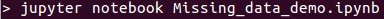
\includegraphics[width=0.5\textwidth]{ipython.png}
\end{figure}
\end{frame}
%------------------------------------------------
\begin{frame}
\frametitle{References}
\footnotesize{
\begin{thebibliography}{9} % Beamer does not support BibTeX so references must 
\bibitem[Wiki, C4.5]{p1}C4.5: \url{https://en.wikipedia.org/wiki/C4.5_algorithm}
\bibitem[Missing Data Analysis]{p2}Missing Data Analysis: \url{https://www.youtube.com/watch?v=QAvSj2TWZy0}
\bibitem[Computerphile]{p3}The Trouble with Missing Data \url{https://www.youtube.com/watch?v=oCQbC818KKU}
\bibitem[Allison, SAS Global Forum 2012]{p4} \textit{Handling Missing Data by Maximum Likelihood}, Paul D. Allison, Statistical Horizons, Haverford, PA, USA
\end{thebibliography}
}
\end{frame}



%----------------------------------------------------------------------------------------

\end{document}